\documentclass[letterpaper,10pt]{article}

\usepackage{mysty}

\begin{document}
\title{COMP9602 Assignment 3}
\author[1]{Zi-Shen Li \thanks{zishen@connect.hku.hk}}
\affil[1]{\it Quantum Information and Computation Initiative, Department of Computer Science, The University of Hong Kong, Hong Kong, China}
\date{\today}
\maketitle

\section{Analysis}\label{sec:analysis}

The target of the problem is to find the best $\vec a=(a_0,a_1,a_2,\cdots,a_{T-1})$ to minimize the energy use of the whole process.
Thus the natrual choice of the original optimization problem is to minimize the energy use of each time step, i.e.
\begin{align}
    E(\vec a)=\sum_{i=0}^{T-1} \phi(a_i),
\end{align}
where $\phi: \Reals_+ \mapsto \Reals_+$ is the energy profile function of a single time step.
In the problem the function $\phi$ is defined to be a convex, increasing function, which also makes the function $E: \Reals_+^T \mapsto \Reals_+$ a convex function because for any $p\in [0,1]$,
\begin{align}
    \label{eq:step1-cvxfunc}E\left[p\vec a+(1-p)\vec b\right] &= \sum_{i=0}^{T-1} \phi[p a_i+(1-p)b_i]\\
    \label{eq:step2-cvxfunc}&\le p\sum_{i=0}^{T-1} \phi(a_i)+(1-p)\sum_{i=0}^{T-1} \phi(b_i)\\
    &=p E(\vec a)+(1-p) E(\vec b),
\end{align}
where from \Cref{eq:step1-cvxfunc} to \Cref{eq:step2-cvxfunc} we have used the convexity of function $\phi$.

The technical difficulty of the problem is its constraint.
First, we directly write down the constraint in the original form
\begin{equation}
    \label{eq:original-constraint}
    \left\{
    \begin{array}{llll}
        & a_i \in [0, a_{\rm max}], & \forall i\in \{0,1,\cdots,T-1\},\\
        & v_{i+1} = v_i + a_i - g, & \forall i\in \{0,1,\cdots,T-1\},\\
        & y_{i+1} = y_i + v_i, & \forall i\in \{0,1,\cdots,T-1\},\\
        & y_{t} \in [l_t, h_t], & \forall t\in \{0,1,\cdots,T\},
    \end{array}\right.
\end{equation}
where $g$ is the acceleration of gravity and $a_{\rm max}$ is the maximum vertical acceleration of the drone.
By utilizing \Cref{eq:original-constraint}, we can rewrite the formula for $y_t$ explicitly in $v_i$
\begin{equation}
    \begin{split}
        y_0 &= y_{\rm init},\\
        y_t &= y_{t-1} + v_{t-1},\\
        y_{t-1} &= y_{t-2} + v_{t-2},\\
        &\cdots\\
        y_1 &= y_0 + v_0,
    \end{split}
\end{equation}
which can be further rewritten as
\begin{align}
    \label{eq:yt}
    y_t = y_0 + \sum_{i=0}^{t-1} v_i,~\forall t\in \{0,1,\cdots,T\}.
\end{align}
In addition, we can also rewrite the formula for $v_t$ explicitly in $a_i$
\begin{equation}
    \begin{split}
        v_t &= v_{t-1} + a_{t} - g,\\
        v_{t-1} &= v_{t-2} + a_{t-1} - g,\\
        &\cdots\\
        v_1 &= v_0 + a_1 - g,\\
        v_0 &= v_{-1} + a_0 - g,\\
        v_{-1} &= 0,
    \end{split}
\end{equation}
which can be further rewritten as
\begin{align}
    \label{eq:vt}
    v_t = \sum_{i=0}^{t} a_i - g t,~\forall t\in \{0,1,\cdots,T-1\}.
\end{align}

Combining \Cref{eq:yt,eq:vt}, we can rewrite $y_t$ explicitly in $a_i$
\begin{align}
    \label{eq:yt-rewrite}
    y_t = y_0 + \sum_{i=0}^{t-1} \left(\sum_{j=0}^{i} a_j - g i\right),~\forall t\in \{1,\cdots,T\}.
\end{align}
More specifically, for $t\in \{1,\cdots,T\}$, we have
\begin{equation}
    y_t=y_0+\sum
    \left\{
        \begin{array}{lllll}
            & a_0\\
            & a_0+a_1-g\\
            & a_0+a_1+a_2-2g\\
            & \cdots\\
            & a_0+a_1+\cdots+a_{t-1}-(t-1)g
        \end{array}
    \right..
\end{equation}
The above formula can be further simplified as
\begin{align}
    y_t &= y_0 + t a_0 + (t-1)a_1 + \cdots + a_{t-1} - \frac{t(t-1)}{2} g\\
    \label{eq:yt-rewrite2}
    &= y_0 + \sum_{j=0}^{t-1} (t-j) a_j - \frac{t(t-1)}{2} g,~\forall t\in \{1,\cdots,T\}.
\end{align}
For any given $y_t$, we can rewrite \Cref{eq:yt-rewrite2} in the form of linear map, i.e.
\begin{align}
    \label{eq:yt-liear-combine}
    y_t = \vec c_t^T \vec a + b_t,
\end{align}
where $\vec c_t\in \Reals^T$ is a column vector with the $(j+1)$-th entry being $(t-j),~\forall j<t$ and $0$ otherwise, and the second term $b_t$ is equal to $y_0-\frac{t(t-1)}{2} g$.
Furthermore, we can vectorize \Cref{eq:yt-liear-combine} to obtain
\begin{align}
    \label{eq:yt-liear-map}
    \vec y = C \vec a + \vec b,
\end{align}
where $\vec y=(y_1,y_2,\cdots,y_T)^T$, and $C$ is a $T\times T$ matrix with the $t$-th row being $\vec c_t^T$.
Note that the matrix $C$ is a lower triangular matrix with all diagonal entries being $1$.
Thus the matrix $C$ is invertible and its inverse matrix is also a lower triangular matrix with all diagonal entries being $1$.
Therefore, we can rewrite \Cref{eq:yt-liear-map} as
\begin{align}
    \label{eq:yt-liear-map2}
    \vec a = C^{-1} (\vec y - \vec b).
\end{align}

The constraint in \Cref{eq:original-constraint} can be rewritten as
\begin{align}
    \label{eq:linear-map-constraint}
    \left\{
    \begin{array}{ll}
        & 0\preceq \vec a \preceq a_{\rm max}\mathds{1},~\mathds{1}:=(1,1,1,\cdots,1)^T,\\
        & \vec l\preceq C \vec a + \vec b \preceq \vec h,
    \end{array}\right.
\end{align}
where $\preceq$ means element-wise inequality. $\vec l$ and $\vec h$ are lower and upper bounds of the height of the drone, respectively.

\section{Solution}

\subsection*{(a)}

The original optimization problem can be rewritten as
\begin{align}
    \min_{\vec a}~ &E(\vec a) = \sum_{i=0}^{T-1} \phi(a_i),\\
    \label{eq:acc-constraint}
    \text{ s.t. } &0\preceq \vec a \preceq a_{\rm max}\mathds{1},\\
    \label{eq:height-constraint}
    &\vec l\preceq C \vec a + \vec b \preceq \vec h.
\end{align}
Or equivalently, we can rewrite \Cref{eq:height-constraint} as
\begin{align}
    \label{eq:height-constraint2}
    &\vec l - \vec b \preceq C \vec a \preceq \vec h - \vec b.
\end{align}
We can show that the above constraints are convex.
Considering $\vec a_1, \vec a_2\in \Reals^T$ and $p\in \Reals$, we have
\begin{align}
    C (p \vec a_1 + (1-p) \vec a_2) &= p C \vec a_1 + (1-p) C \vec a_2,
\end{align}
and we assume $a_1,a_2$ satisfy the constraints in \Cref{eq:height-constraint2}, i.e., $\vec l_1 - \vec b \preceq C \vec a_1 \preceq \vec h_1 - \vec b$ and $\vec l_2 - \vec b \preceq C \vec a_2 \preceq \vec h_2 - \vec b$.
It is easy to see that the convex combination of $\vec a_1$ and $\vec a_2$ also satisfies the constraints, i.e.,
\begin{align}
    \vec l_1 - \vec b \preceq C (p \vec a_1 + (1-p) \vec a_2) \preceq \vec h_1 - \vec b.
\end{align}
The result still holds for the constraint in \Cref{eq:acc-constraint} for the same reason.

As we shown in \Cref{sec:analysis}, the function $E(\vec a)$ is convex.
Thus we can conclude the optimization problem is a convex problem.

\subsection*{(b)}

The energy profile $\phi$ is given by
\begin{align}
    \phi(a)=1+a+a^2+a^3.
\end{align}
We aim to solve the optimization problem with ellipsoid method.
The objective function can be written as
\begin{align}
    E(\vec a)=\sum_{i=0}^{T-1} \phi(a_i)=T+\sum_{i=0}^{T-1} a_i + \sum_{i=0}^{T-1} a_i^2 + \sum_{i=0}^{T-1} a_i^3,
\end{align}
which are differentiable.
Thus the subgradient of $E(\vec a)$ is the gradient of $E(\vec a)$, i.e.,
\begin{align}
    \frac{\partial E}{\partial a_i} = 1 + 2a_i + 3a_i^2.
\end{align}
The gradient of the constrain in \Cref{eq:height-constraint2} is also differentiable, i.e.,
\begin{align}
    \nabla_{\vec a} (C \vec a) = C^T.
\end{align}
For each constrain in \Cref{eq:yt-liear-combine}, we have $\forall t\in \{1,\cdots,T\}$,
\begin{align}
    &f_{1t}=\vec c_t^T \vec a + b_t -h_t\le 0,\\
    &f_{2t}=l_t - \vec c_t^T \vec a - b_t\le 0,
\end{align}
where $b_t=y_0-\frac{t(t-1)}{2}g$, and additionally, we have
\begin{align}
    &f_{3t}=-a_{\rm max} + a_t \le 0,\\
    &f_{4t}=- a_t \le 0.
\end{align}
The gradient of the above two sets of constrains are
\begin{align}
    &\nabla_{\vec a} f_{1t}=\vec c_t,\\
    &\nabla_{\vec a} f_{2t}=-\vec c_t,\\
    &\nabla_{\vec a} f_{3t}=\vec e_t,\\
    &\nabla_{\vec a} f_{4t}=-\vec e_t,
\end{align}
where $\vec c_t=(t, t-1, \cdots, 1, 0, \cdots, 0)^T$ is a column vector with the first $t$ entries being $t, t-1, \cdots, 1$ and the rest being $0$, and $\vec e_t$ is a column vector with the $t$-th entry being $1$ and the rest being $0$.

\subsection{(c)}

All codes of the programe as well as the LaTeX codes are provided in the link \href{https://github.com/Zi-Shen/cvx-a3}{github.com/Zi-Shen/cvx-a3}
, which is currently a private repository but will be made public after the deadline of the assignment. The sourse codes are written in Python 3.9 and it can be found in the directory \texttt{src/main.py}. The source codes are also be submitted accompanying with this report.

\subsubsection*{Instance 1}

The first instance is a trivial case where the optimal solution is letting the drone turn off its engine during the whole process. The result and required informations are provided in \Cref{fig:instance1}.
The optimal objective function value provided by the programe is (keep 12 significant digits)
\begin{align}
    E(\vec a^*)\approx 2.00054077480.
\end{align}

\subsubsection*{Instance 2}

The second instance is a more complicated case where the drone needs to tuning its engine to manipulate its height. 
The result and required informations are provided in \Cref{fig:instance2}.
The optimal objective function value provided by the programe is (keep 12 significant digits)
\begin{align}
    E(\vec a^*)\approx 35951.8168589.
\end{align}

\begin{figure}
    \centering
    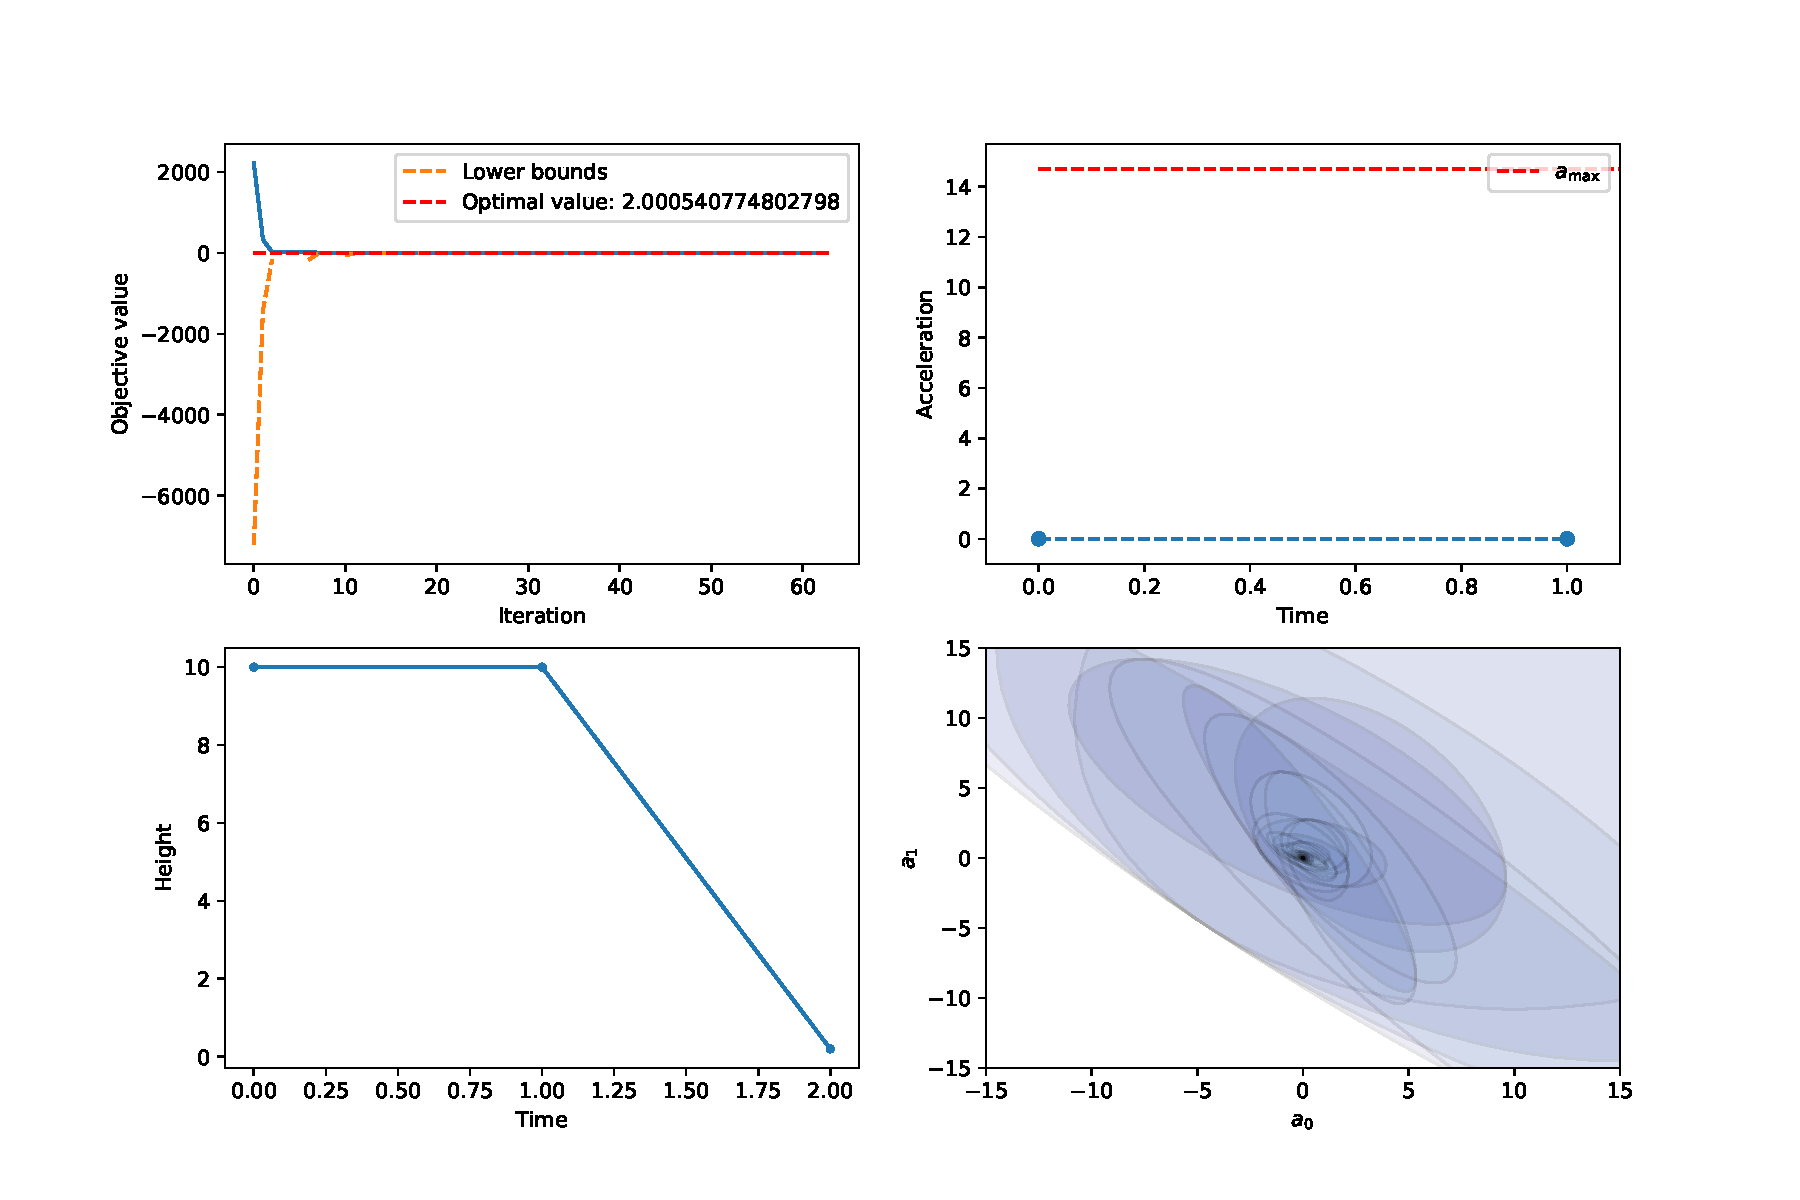
\includegraphics[width=0.9\textwidth]{fig/Figure_1.pdf}
    \caption{\textbf{Instance 1}. The drone turns off its engine and undergoes a parabolic trajectory. Lower-right figure shows evolution of the ellipsoid during the optimization process.}
    \label{fig:instance1}
\end{figure}

\begin{figure}
    \centering
    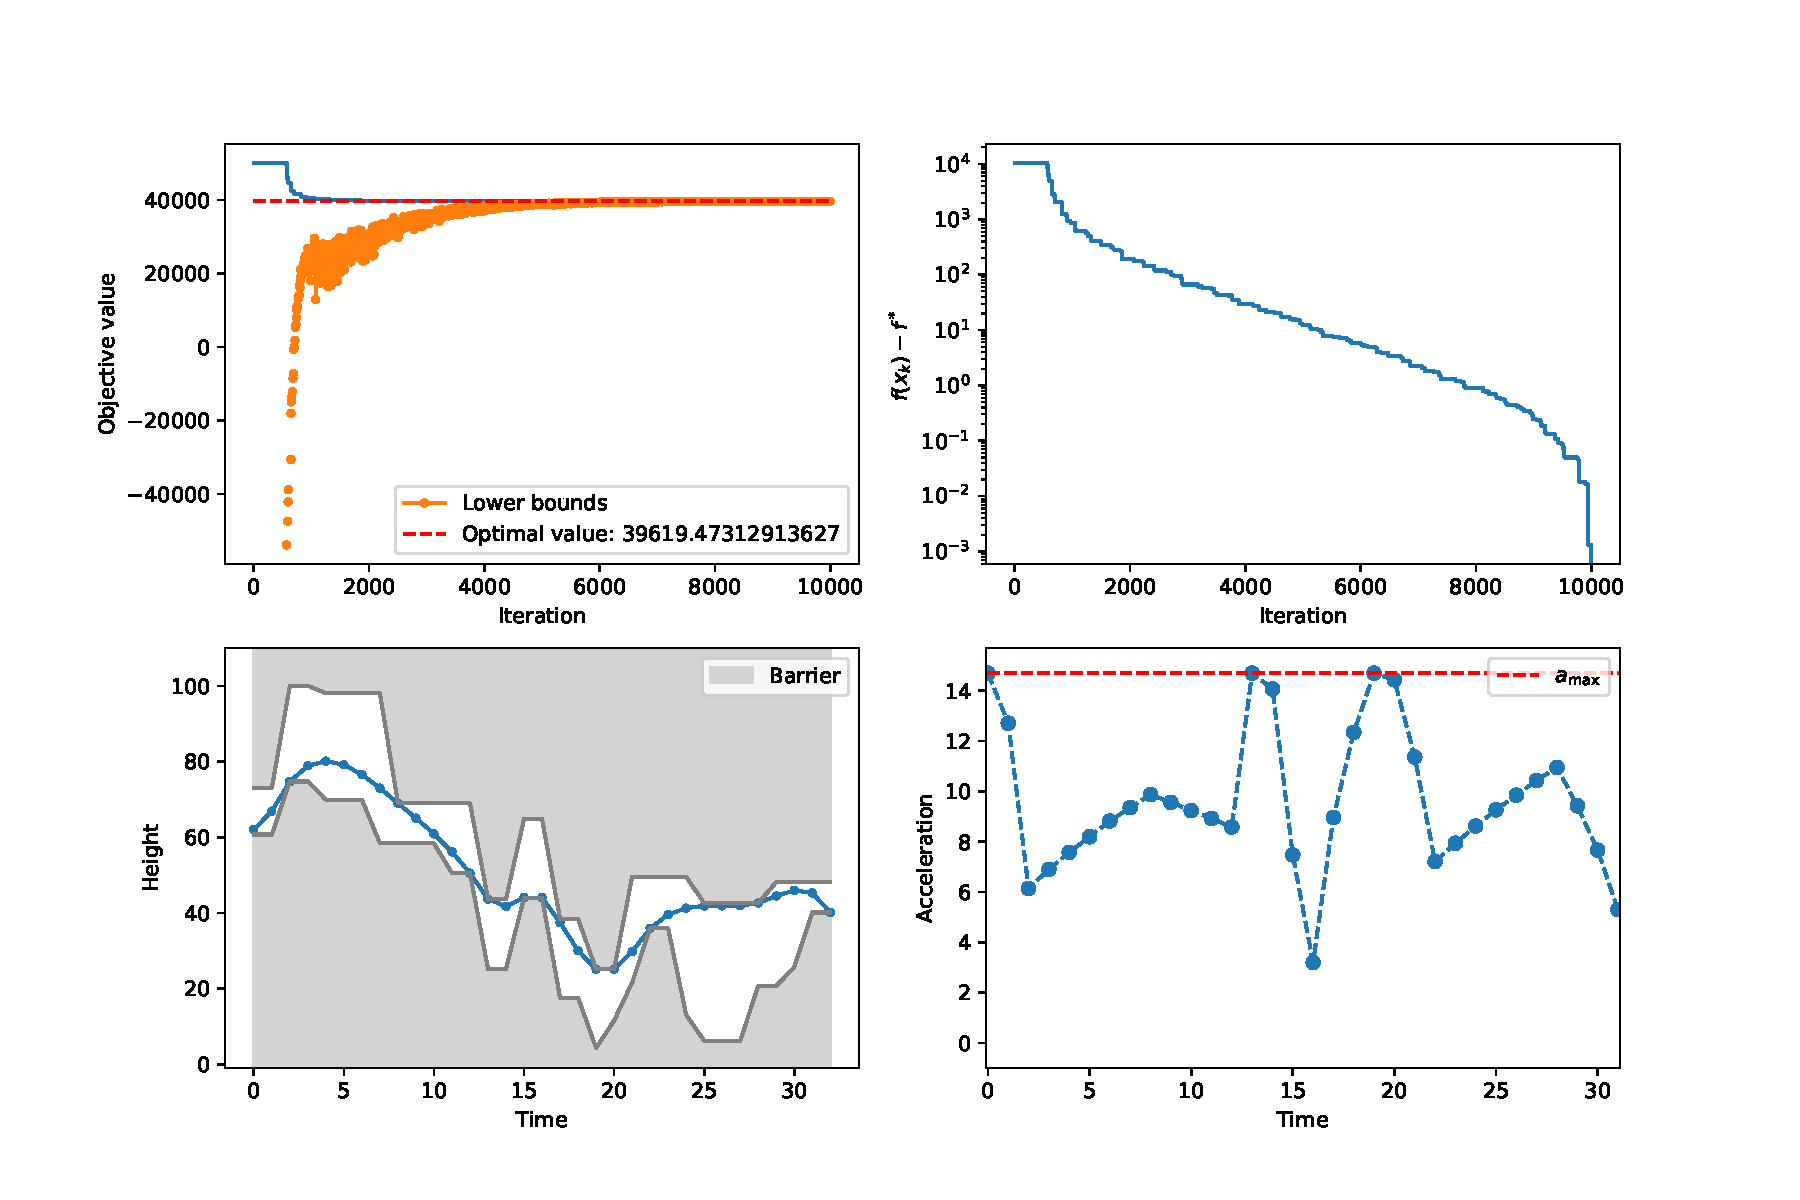
\includegraphics[width=0.9\textwidth]{fig/Figure_2.pdf}
    \caption{\textbf{Instance 2}. The drone avoids obstacles through a series of complex operations. Upper-right figure shows how the objective function converges in the log scale.}
    \label{fig:instance2}
\end{figure}

\end{document}